\section{System Architecture}\label{sec:arch}

\begin{figure*}[t]
\centering
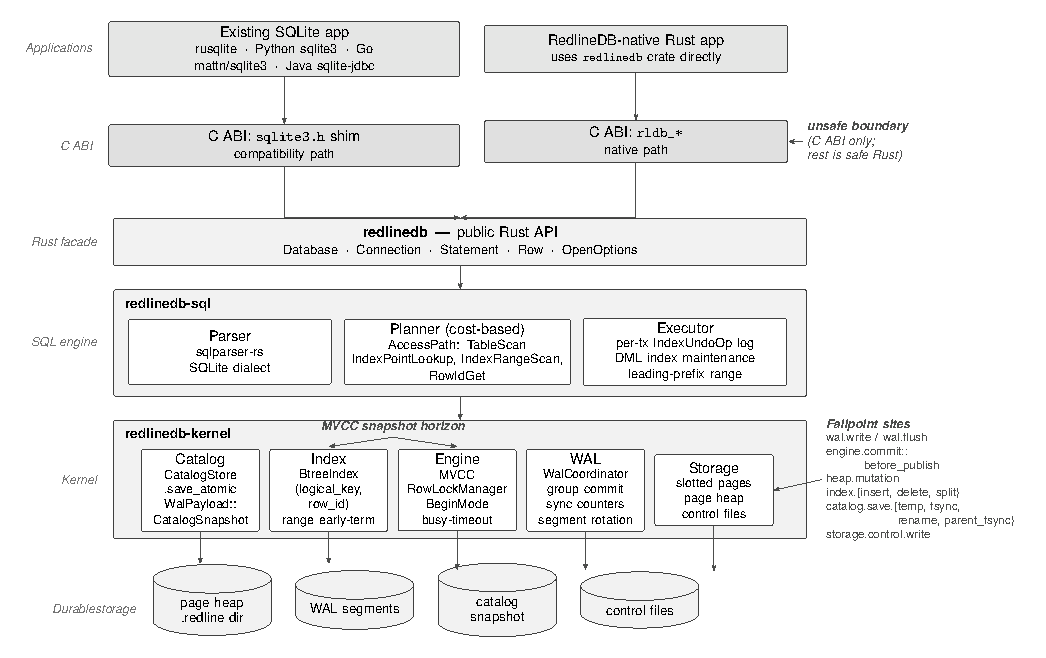
\includegraphics[width=2\columnwidth]{figs/architecture.eps}
\caption{RedlineDB layered architecture. The five horizontal bands are
the C ABI shim (\texttt{sqlite3.h}), the native \texttt{rldb\_*} FFI,
the public Rust facade (\texttt{redlinedb}), the SQL layer
(parser/planner/executor), and the kernel (catalog, engine, index,
storage, WAL). The right-hand annotations identify the
\texttt{unsafe} boundary (only inside \texttt{ffi}) and the
fail-point sites threaded through WAL, commit publish, heap
mutation, index mutation, and catalog rename. The bottom row is the
durable substrate: page-heap segments, WAL segments, catalog
snapshot, and control files.}
\label{fig:arch}
\end{figure*}

Figure~\ref{fig:arch} shows the layered architecture. The repository
splits into five Cargo crates:
\texttt{redlinedb-kernel} (catalog, engine, index, page heap, WAL,
storage), \texttt{redlinedb-sql} (parser, planner, executor),
\texttt{redlinedb} (the public Rust facade and registry),
\texttt{redlinedb-ffi} (C ABI surface), and \texttt{redlinedb-bench}
(the certification harness). Crate boundaries match the layering of
Figure~\ref{fig:arch}: kernel below, SQL on top, facade above SQL, FFI
above facade. The dependency graph is acyclic and the kernel has no
SQL dependency, which lets the kernel be tested in isolation against
the same fail-point grammar that the harness drives.

\subsection{Storage: Slotted Heap Pages and Recursive Footprint}
The page heap is a slotted-page store with a 16~KiB page size. Each
page carries a header, a slot directory, and a tuple region; a tuple
slot stores either a live tuple, a forwarding pointer (when an update
grows past the in-place slot), or a tombstone gated by an MVCC
visibility CSN. The slotted layout~\cite{bayer1972btree} gives us
in-page rearrangement without rewriting external pointers: an update
that fits the existing slot writes in place, while one that does not
allocates a fresh slot on the same or a sibling page and leaves a
forwarding pointer behind. Free space within a page is reclaimed via
vacuuming during the next compaction pass. The on-disk footprint is
reported through a recursive walker (the bench harness uses
\texttt{walkdir} to sum every byte under the database directory,
including WAL segments, catalog snapshots, and the rolled-archive
segment store) so that any size regression caused by leaked pages,
orphaned WAL segments, or stale snapshots shows up as a delta on the
next certification run.

\subsection{MVCC and Version Chains}
Each row carries a per-row version chain keyed by the writing
transaction's commit sequence number (CSN). A reader at snapshot
$t_r$ walks the chain from the head and selects the latest version
whose commit-CSN is at or before $t_r$. Live (uncommitted) versions
are stamped with the writer's transaction ID and become visible only
when the writer publishes a CSN at commit. Aborted versions are
elided by the next visibility scan; a background vacuum pass reclaims
their slots. This is the standard MVCC discipline of
Bernstein and Goodman~\cite{bernstein1983mvcc} and matches the
production patterns of PostgreSQL~\cite{postgresql_mvcc} and
InnoDB~\cite{innodb_mvcc}.

\subsection{WAL: Group Commit and Sync Counters}
The kernel exposes a \texttt{WalCoordinator} that mediates writes
into a sequence of WAL segments. Group commit batches transactions
that arrive within a small window onto a single \texttt{fsync},
amortizing the durability cost across writers. The coordinator
threads two pass-through counters (fdatasync count and pwrite count)
out to the bench harness so each per-thread row in the harness output
carries the durability cost of that run. Recovery replays redo
records up to the last durable LSN and uses the per-record undo
chain to roll back transactions that did not commit.
The catalog is durable through a dual mechanism: an atomic on-disk
snapshot (\texttt{save\_atomic} writes to a temp file and renames
under a parent directory \texttt{fsync}) and a
\texttt{WalPayload::CatalogSnapshot} record that carries the same
bytes through the WAL. On recovery, the WAL snapshot wins if it is
newer than the on-disk file.

\subsection{Indexes: B-link Lifecycle, $(\mathrm{key}, \mathrm{rowid})$ Physical Key}
The index layer is a B$^+$-tree with the
B-link discipline~\cite{lehman1981blink,srinivasan1991bplus}. The
physical key is the tuple $(\mathrm{logical\_key}, \mathrm{row\_id})$ rather
than just $\mathrm{logical\_key}$. This handles duplicate runs cleanly:
two rows with the same logical key occupy adjacent leaf slots, and a
range scan that hits the upper bound terminates as soon as the
\texttt{logical\_key} component exceeds the bound (early termination
sidesteps the duplicate-key tail). Index mutations are transactional:
\texttt{insert\_tx} marks an entry as live-but-uncommitted,
\texttt{delete\_mark\_tx} marks an entry as dead-but-uncommitted, and
\texttt{undelete\_mark\_tx} (introduced for rollback) re-clears the
dead flag. None of these operations physically remove a slot during a
live transaction, so undo never has to reconstruct a deleted entry.

\subsection{Concurrency: Row Locks, Snapshots, Begin Modes}
A \texttt{RowLockManager} serializes writers contending on the same
row using relation-aware keys: the lock key is
$(\mathrm{table\_id}, \mathrm{row\_id})$, never just $\mathrm{row\_id}$, so
that two tables with overlapping rowid spaces never share a lock. The
manager is hierarchically organized in the spirit of Gray's
granularity-of-locks framework~\cite{gray1976granularity}; row locks
are the only granule at runtime, but the design space leaves room
for table-granule extensions when DDL serializes across writers.
The lock supports a configurable busy timeout that mirrors SQLite's
\texttt{busy\_timeout} semantics: a contender waits up to the timeout
before returning a \texttt{BUSY}-class error. The harness records
\texttt{BUSY}, \texttt{LOCKED}, and \texttt{TIMEOUT} as separate
counters per run so that a workload's contention shape can be read
off the certification output directly rather than inferred from a
combined error rate. The
\texttt{BeginMode} enum exposes \texttt{Deferred}, \texttt{Immediate},
and \texttt{Exclusive} starts, again matching SQLite's
\texttt{BEGIN}/\texttt{BEGIN IMMEDIATE}/\texttt{BEGIN EXCLUSIVE}
contract. Read-only transactions never enter the row-lock manager;
they take an MVCC snapshot via the CSN allocator and never block.
Disjoint-row writers proceed in parallel by construction. This is
how RedlineDB removes the single-writer WAL ceiling without changing
the user-facing transaction model.

\subsection{Planner: Cost-Based AccessPath, Honest EXPLAIN}
The planner consumes a \texttt{sqlparser} AST and emits an
\texttt{AccessPath} that the executor can drive directly:
\texttt{TableScan}, \texttt{IndexPointLookup}, \texttt{IndexRangeScan},
or \texttt{RowIdGet}. The planner-executor invariant
\texttt{access\_path\_is\_consumable\_by\_executor} is checked
before the path is shipped to execution: if the catalog entry for an
index is missing a \texttt{meta\_page\_id}, or if the engine has no
live handle for it, the planner refuses to advertise that path and
the executor falls back to a table scan. The result is that
\texttt{EXPLAIN} never lies about which index will run.

\subsection{Executor: Per-Tx Index Undo, NULL Skip Parity}
DML executes through \texttt{execute\_insert}, \texttt{execute\_update},
and \texttt{execute\_delete}. Each maintains a per-transaction
\texttt{IndexUndoOp} log: every B-link mutation that the executor
issues is paired with the inverse op the kernel will need if the
transaction rolls back, or---critically---if commit itself fails after
the kernel has already mutated indexes. On commit failure, the
executor replays the undo log against the live index handles, then
the kernel transitions the transaction to \texttt{Aborted}. We follow
SQLite's NULL-skip rule for unique constraints: a row whose unique
key contains a NULL is allowed to coexist with other such rows,
because NULL is not equal to NULL.

\subsection{FFI: rldb\_* Native and sqlite3.h Compatibility}
The FFI crate exposes two C surfaces. The native surface is a small
\texttt{rldb\_*} ABI that maps directly onto the public Rust facade.
The compatibility surface is a \texttt{sqlite3.h} header whose
covered symbols (\texttt{sqlite3\_open\_v2}, \texttt{sqlite3\_prepare\_v2},
\texttt{sqlite3\_step}, \texttt{sqlite3\_column\_*}, \texttt{sqlite3\_finalize},
\texttt{sqlite3\_close}) are routed through the same kernel paths.
This crate is the only one in the workspace where \texttt{unsafe}
appears at any density, and the unsafe blocks exist because the C
calling convention requires them.
